% !TeX spellcheck = en_US

\chapter{Check}\label{chap:check}
In this chapter, the developed framework will be checked.
The output CSAR will be added to and displayed by \nameref{subs:wine}.
Generated Artifacts will be checked in command line.
\if 0 
%TODO
надо прописать какой именно архив использовался и какие в нём зависимости
потом установить как то хз как
\fi
\section{Check by Winery}
 \nameref{subs:wine} was installed to test the correctness of output CSAR. 
 This is an environment for development TOSCA systems and is useful for checking results. \\
 The INSERT NAME from INSERT ADDRESS will be used as a source CSAR. 
 His representation in winery is displayed on figure \ref{fig:winery_source2}.
\begin{figure}[ht]   
	\centering
	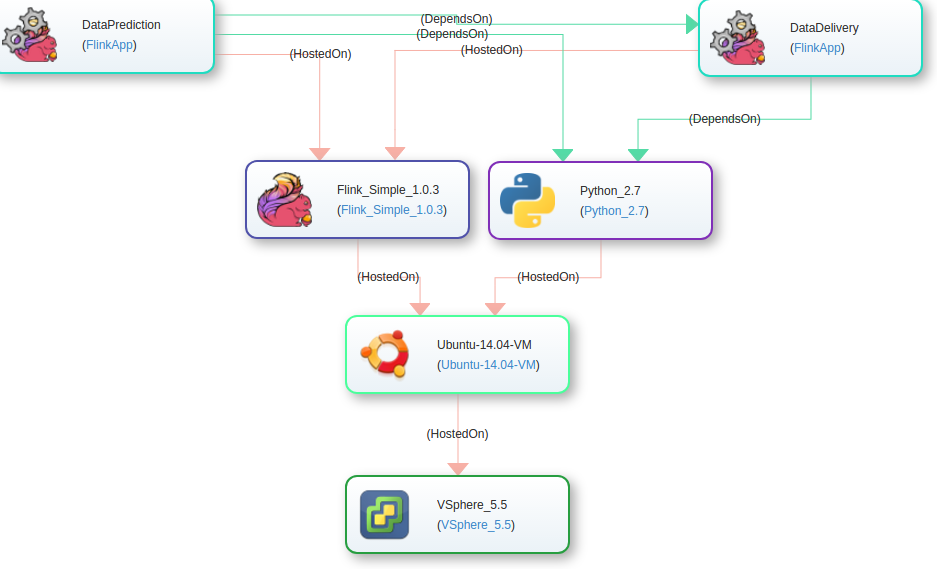
\includegraphics[width=0.7\textwidth]{Screenshot_winery_source2}
	\caption{Source CSAR represented by $Winery$.}
	\label{fig:winery_source2}
\end{figure}
 This CSAR has a purely simple structure.
 Flink Simple Application has a two submodules: Data Prediction and DataDelivery, both a hosted on Flink Simple Platform and require Python2.7. 
 That all runs over Ubuntu 14.
 Deep analysis shows that Flink Simple Platform installs java and node Python2.7 installs program python2.7.
 Those external references are resolved during processing by the framework and exchanged by new nodes in output CSAR.
 This output CSAR will be added to Winery.
 Due to significant increase in size, this can be a fairly lengthy procedure.
 There where 10 nodes in source CSAR, then after processing bz the framework, there are already more then 100 of nodes.
 During the addition, a CSAR's syntax is tested.
 In case of errors, messages will be displayed.
 Then Service Template will be displayed.
 Again, due to high number of nodes, preprocessing can take a long time. 
 But at the time, the correctness of the links will be checked.
 If something was defined not properly, the nodes or links between them will not be displayed.
Representation of the output CSAR in the winery is shown on figure \ref{fig:winery_output} (Only a part of CSAR is visible).
\begin{figure}[ht]   
	\centering
	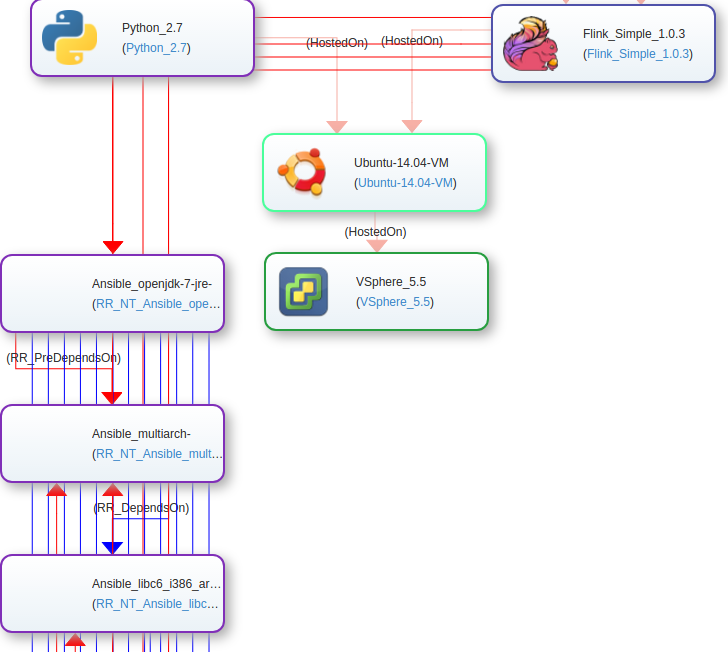
\includegraphics[width=0.7\textwidth]{Screenshot_winery_output}  
	\caption{Output CSAR represented by $Winery$.}
	\label{fig:winery_output}
\end{figure}
 It seems pretty beloved.
 To verify the TOSCA's structure some nodes was moved manually (figure \ref{fig:winery_output2}). 
 \begin{figure}[ht]   
 	\centering
 	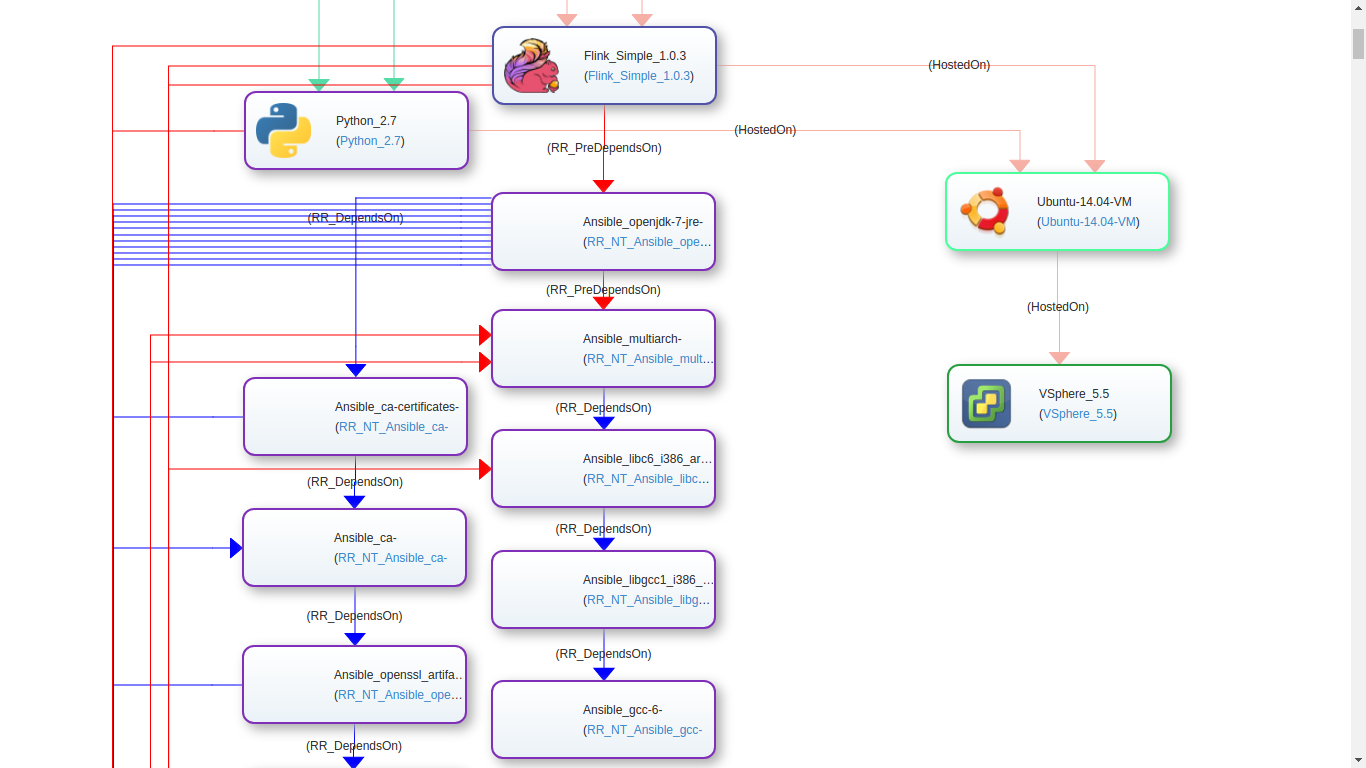
\includegraphics[width=0.7\textwidth]{Screenshot_winery_output2}
 	\caption{Output CSAR represented by $Winery$, nodes manually moved.}
 	\label{fig:winery_output2}
 \end{figure}
 By checking several nodes with $apt$-$cache$ $depends$ command, the correctness of dependencies can be verified.
 By opening the content of the new nodes, it can be verified, that the are scripts and packages for installation.

\section{Check installations}
Also is is necessary to check whether it is possible to install new packages using the generated installation scripts.
First bash scripts will be tested, then ansible playbooks.
\subsection{Check bash scripts}
Since bash is used in Linux's command line it will be pretty easy to check bash installation scripts by starting them (of course that must be done having necessary privileges).
Example of python2.7 installation is presented in Listing \ref{lst:check_bash_script}.\\
\begin{Listing}
\caption{Check bash installation script}
\label{lst:check_bash_script}
\begin{lstlisting}
user@user:~$ sudo ./RR_python2_7-minimal.sh 
(Reading database ... 286091 files and directories currently installed.)
Preparing to unpack python2_7-minimal.deb ...
Unpacking python2.7-minimal (2.7.12-1ubuntu0~16.04.1) over (2.7.12-1ubuntu0~16.04.1) ...
Setting up python2.7-minimal (2.7.12-1ubuntu0~16.04.1) ...
Processing triggers for man-db (2.7.5-1) ...
\end{lstlisting}
\end{Listing}
Since the process ended without warnings and errors, it was completed successfully.
This way every bash installation script can be checked.

\subsection{Check ansible playbooks}
To check ansible playbook manually we need to extract zip file containing playbook. 
During regular execution this work must be done by runtime environment.
Calling ansible runtime to proceed the playbook is a simple procedure too.
Example is provided on figure \ref{fig:ansible_output2}.\\
 \begin{figure}[ht]   
	\centering
	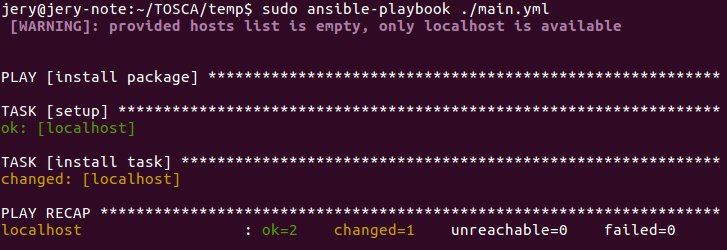
\includegraphics[width=0.7\textwidth]{Screenshot_ansible_output}
	\caption{Ansible playbook execution process}
	\label{fig:ansible_output2}
\end{figure}
$Ok$ signals that the installation was successfully completed.